\documentclass[xetex]{beamer}
\usepackage{fontspec}
\usepackage{arev}
\usepackage{mathtools}
\usepackage{unicode-math}
\usepackage{tikz}
\usetikzlibrary{trees}
\usepackage{mathpartir}
\usepackage{parskip}
\usepackage{empheq}
\usepackage{minted}
\usepackage{csquotes}
\usepackage{tcolorbox}
\usepackage{biblatex}
\usepackage[normalem]{ulem}

\setmainfont{XITS}
\setsansfont{DejaVu Sans}
\setmathfont{XITS Math}
\setmonofont{DejaVu Sans Mono}

\addbibresource{lit.bib}

% Emoji images are from
% https://github.com/joypixels/emoji-assets/blob/master/png/128
\newlength{\emojiheight}
\settoheight{\emojiheight}{H}
\newcommand{\good}{
\includegraphics[height=\emojiheight]{images/1f973}}
\newcommand{\bad}{
\includegraphics[height=\emojiheight]{images/1fae4}}

\setbeamertemplate{navigation symbols}{}
\setbeamertemplate{itemize item}{\Large\textbullet}
\setbeamertemplate{itemize subitem}{\Large\textbullet}
\setbeamertemplate{itemize subsubitem}{\Large\textbullet}

\tcbset{frame empty}

\newmintinline[lean]{lean4}{bgcolor={},ignorelexererrors=true}
\newminted[leancode]{lean4}{bgcolor={},ignorelexererrors=true,fontsize=\footnotesize,autogobble}
\BeforeBeginEnvironment{leancode}{\begin{tcolorbox}}
\AfterEndEnvironment{leancode}{\end{tcolorbox}}
\usemintedstyle{tango}

\setlength{\parskip}{1em}
\setlength{\tabcolsep}{0.5em}

% Source: https://tex.stackexchange.com/questions/55806/mindmap-tikzpicture-in-beamer-reveal-step-by-step/55849#55849
%
% Keys to support piece-wise uncovering of elements in TikZ pictures:
% \node[visible on=<2->](foo){Foo}
% \node[visible on=<{2,4}>](bar){Bar}   % put braces around comma expressions
%
% Internally works by setting opacity=0 when invisible, which has the
% advantage (compared to \node<2->(foo){Foo} that the node is always there, hence
% always consumes space plus that coordinate (foo) is always available.
%
% The actual command that implements the invisibility can be overridden
% by altering the style invisible. For instance \tikzsset{invisible/.style={opacity=0.2}}
% would dim the "invisible" parts. Alternatively, the color might be set to white, if the
% output driver does not support transparencies (e.g., PS)
\tikzset{
  invisible/.style={opacity=0},
  visible on/.style={alt={#1{}{invisible}}},
  alt/.code args={<#1>#2#3}{%
    \alt<#1>{\pgfkeysalso{#2}}{\pgfkeysalso{#3}} % \pgfkeysalso doesn't change the path
  },
}

\renewcommand{\iff}{\leftrightarrow}
\newcommand{\com}{,\,}
\newcommand{\orange}[1]{\textcolor{orange}{#1}}
\newcommand{\blue}[1]{{\usebeamercolor[fg]{palette primary} #1}}
\newcommand{\grey}[1]{\textcolor{lightgrey}{#1}}
\newcommand{\mv}[1]{\ensuremath{\mathit{?#1}}}
\newcommand{\rulename}[1]{\textrm{#1}}
\newcommand{\rulelabel}[1]{\quad \text{\rulename{#1}}}
\newenvironment{rapppic}{\begin{tikzpicture}[outer sep=auto, level distance=2em]}{\end{tikzpicture}}
\newenvironment{rapp}{%
  \begin{tcolorbox}
  \begin{center}
  \begin{rapppic}
}{
  \end{rapppic}
  \end{center}
  \end{tcolorbox}%
}

\begin{document}

\title{Aesop: White-Box Automation for Lean~4}
\author{Jannis Limperg\\ University of Munich (LMU)\\ \href{mailto:jannis@limperg.de}{jannis@limperg.de}}
\date{TODO}

\begin{frame}
  \maketitle
\end{frame}

\begin{frame}
  \tableofcontents
\end{frame}

\AtBeginSection{
  \begin{frame}
    \usebeamercolor[fg]{frametitle}
    \Large \center{\insertsection}
  \end{frame}
}

\section{Search Algorithm}

\begin{frame}
  \frametitle{Rules}

  A \emph{rule} is an arbitrary Lean tactic.

  Aesop provides convenient syntax (\emph{rule builders}) for creating rules from theorems.

  Aesop always operates with a user-defined \emph{rule set}.
\end{frame}

\begin{frame}[fragile]
  \frametitle{Basic Tree Search}

  \begin{center}
    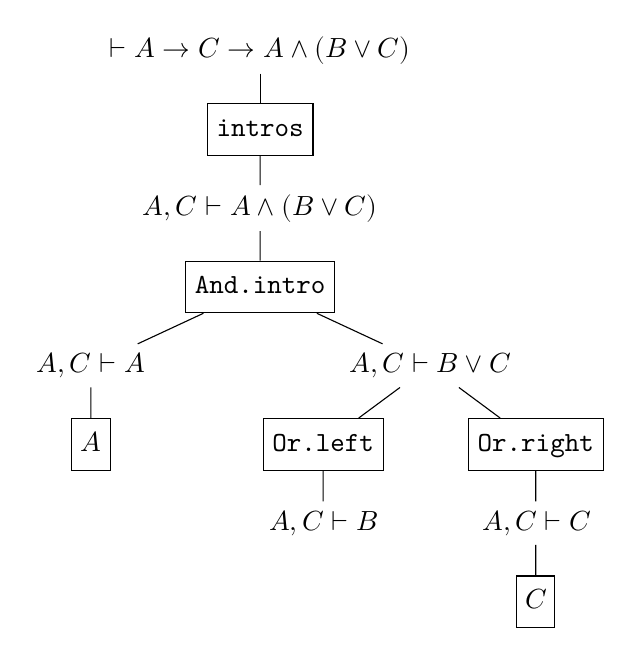
\begin{tikzpicture}[outer sep=auto, level distance=10mm]
      \node {$⊢ A → C → A ∧ (B ∨ C)$}
      child[visible on=<2->] {node[rectangle,draw] {\texttt{intros\strut}}
        child[visible on=<2->] {node {$A, C ⊢ A ∧ (B ∨ C)$}
          child[visible on=<3->] {node[rectangle,draw] {\texttt{And.intro\strut}}
            child[visible on=<3->] {node[xshift=-14mm] {$A, C ⊢ A$}
              child[visible on=<4->] {node[rectangle,draw] {$A\strut$}}}
            child[visible on=<3->] {node[xshift=14mm] {$A, C ⊢ B ∨ C$}
              child[visible on=<5->] {node[rectangle,draw,xshift=-6mm] {\texttt{Or.left\strut}}
                child[visible on=<5->] {node {$A, C ⊢ B$}}}
              child[visible on=<6->] {node[rectangle,draw,xshift=6mm]  {\texttt{Or.right\strut}}
                child[visible on=<6->] {node {$A, C ⊢ C$}
                  child[visible on=<7->] {node[rectangle,draw] {$C\strut$}}}}}}}};
    \end{tikzpicture}
  \end{center}
\end{frame}

\newcommand*{\sprob}[1]{\blue{\textrm{#1\%}}}
\newcommand*{\prio}[1]{{\uncover<2->{\orange{\textrm{#1}\%}}}}

\begin{frame}
  \frametitle{Best-First Tree Search}

  \begin{center}
    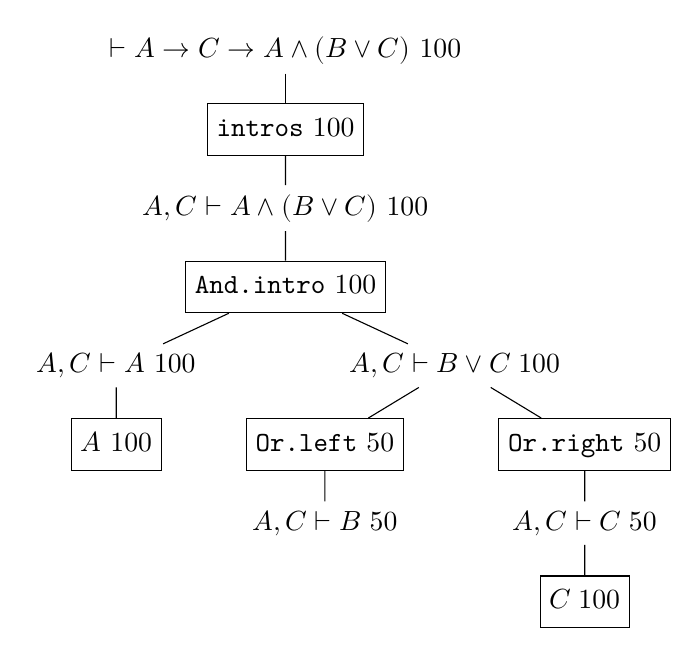
\begin{tikzpicture}[outer sep=auto, level distance=10mm]
      \node {$⊢ A → C → A ∧ (B ∨ C)$ \prio{100}}
      child {node[rectangle,draw] {\texttt{intros\strut} \sprob{100}}
        child {node {$A, C ⊢ A ∧ (B ∨ C)$ \prio{100}}
          child {node[rectangle,draw] {\texttt{And.intro\strut} \sprob{100}}
            child {node[xshift=-14mm] {$A, C ⊢ A$ \prio{100}}
              child {node[rectangle,draw] {$A\strut$ \sprob{100}}}}
            child {node[xshift=14mm] {$A, C ⊢ B ∨ C$ \prio{100}}
              child {node[rectangle,draw,xshift=-9mm] {\texttt{Or.left\strut} \sprob{50}}
                child {node {$A, C ⊢ B$ \prio{50}}}}
              child {node[rectangle,draw,xshift=9mm]  {\texttt{Or.right\strut} \sprob{50}}
                child {node {$A, C ⊢ C$ \prio{50}}
                  child {node[rectangle,draw] {$C\strut$ \sprob{100}}}}}}}}};
    \end{tikzpicture}
  \end{center}
\end{frame}

\begin{frame}
  \frametitle{Safe Rules}

  \begin{itemize}[<+->]
    \item Run before unsafe rules
    \item If a safe rule succeeds on a goal $G$, no other rules are tried for $G$
    \item Integer penalty
    \item Treated as 100\% success probability
    \item \good{} Good for performance
    \item \bad{} Users need to make sure that the rule really is safe
  \end{itemize}
\end{frame}

\begin{frame}[fragile]
  \frametitle{Examples}

  \begin{block}{Safe rule: ∧-introduction}
    \begin{rapp}
      \node {$Γ ⊢ \orange{A ∧ B}$}
        child {node {$Γ ⊢ \orange{A}$}}
        child {node {$Γ ⊢ \orange{B}$}};
    \end{rapp}
  \end{block}

  \begin{block}{Unsafe rule: left ∨-introduction}
    \begin{rapp}
      \node {$Γ ⊢ \orange{A ∨ B}$}
        child {node {$Γ ⊢ \orange{A}$}};
    \end{rapp}
  \end{block}
\end{frame}

\begin{frame}
  \frametitle{When Is A Rule Safe?}

  A rule $R$ is \emph{logically safe} if it preserves provability:

  For each goal $G$, if $G$ is provable and $R$, applied to $G$, generates subgoals $G₁, \dots, Gₙ$, then $G₁, \dots, Gₙ$ must still be provable.

  \pause

  A rule $R$ is \emph{relatively safe} if it preserves provability relative to a rule set $S$:

  If a goal $G$ is provable with rules from $S$ and $R$, applied to $G$, generates subgoals $G₁, \dots, Gₙ$, then $G₁, \dots, Gₙ$ must still be provable with rules from $S$.
\end{frame}

\begin{frame}
  \frametitle{Normalisation Rules}

  \begin{itemize}[<+->]
    \item Run before safe rules
    \item Integer penalty
    \item Treated as 100\% success probability
    \item May produce only one subgoal
    \item Run in a fixpoint loop, i.e.\ until no normalisation rule succeeds any more
    \item \good{} Can establish invariants for other rules
    \item \bad{} Typically run multiple times on every goal
  \end{itemize}
\end{frame}

\begin{frame}
  \frametitle{Example}

  \begin{block}{∧-elimination}
    \begin{rapp}
      \node {$Γ,\, \orange{h : A ∧ B} ⊢ T$}
        child {node {$Γ,\, \orange{h₁ : A},\, \orange{h₂ : B} ⊢ T$}};
    \end{rapp}
  \end{block}
\end{frame}

% Discuss normalisation loop here if there's time.

\begin{frame}[fragile]
  \frametitle{Summary: Aesop's Search Algorithm}

  \begin{center}
    \small
    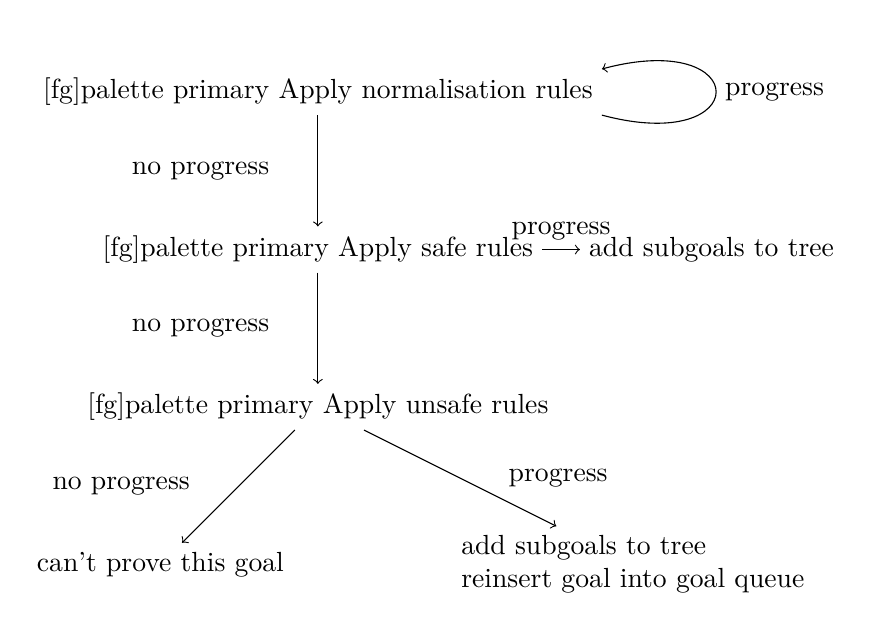
\begin{tikzpicture}[outer sep=auto, norm/.style={}, safe/.style={}, unsf/.style={}]
      \path
        (0,6)  node[norm]            (norm)        {\blue{Apply normalisation rules}}
        (0,4)  node[safe]            (safe)        {\blue{Apply safe rules}}
        (5,4)  node[safe]            (safe-done)   {add subgoals to tree}
        (0,2)  node[unsf]            (unsafe)      {\blue{Apply unsafe rules}}
        (-2,0) node[unsf]            (fail)        {can't prove this goal}
        (4,0)  node[unsf,align=left] (unsafe-done) {add subgoals to tree \\ reinsert goal into goal queue};
      \draw[<-,norm,loop right, min distance=20mm] (norm.{north east}) to node {progress} (norm.{south east});
      \draw[->,safe] (norm) -- node[left,xshift=-5mm] {no progress} (safe);
      \draw[->,safe] (safe) -- node[above] {progress} (safe-done);
      \draw[->,unsf] (safe) -- node[left,xshift=-5mm] {no progress} (unsafe);
      \draw[->,unsf] (unsafe) -- node[left,xshift=-5mm] {no progress} (fail);
      \draw[->,unsf] (unsafe) -- node[right,xshift=5mm] {progress} (unsafe-done);
    \end{tikzpicture}
  \end{center}
\end{frame}

\section{Registering Rules}

\begin{frame}[fragile]
  \frametitle{Registering Rules}

  \begin{block}{Globally}
    \begin{leancode}
      @[aesop unsafe 100%]
      theorem And.intro : A → B → A ∧ B
    \end{leancode}
  \end{block}

  \pause

  \begin{block}{Locally}
    \begin{leancode}
      aesop (add 100% And.intro)
    \end{leancode}
  \end{block}

  \pause

  \begin{block}{Safe rules}
    \begin{leancode}
      @[aesop safe 10]
      theorem And.intro : A → B → A ∧ B
    \end{leancode}
  \end{block}
\end{frame}

\begin{frame}
  \frametitle{Rule Builders}

  A \emph{rule builder} turns a declaration into an Aesop rule.

  In the examples so far, we have implicitly used a default builder.

  Aesop currently provides 7 rule builders.
\end{frame}

\begin{frame}[fragile]
  \frametitle{Apply Builder}

  \begin{leancode}
    @[aesop safe apply 10]
    theorem And.intro : A → B → A ∧ B
  \end{leancode}

  \pause

  Builds a rule that runs \lean{apply And.intro}.

  \begin{rapp}
    \node {$Γ ⊢ \orange{A ∧ B}$}
      child {node {$Γ ⊢ \orange{A}$}}
      child {node {$Γ ⊢ \orange{B}$}};
  \end{rapp}
\end{frame}

\begin{frame}[fragile]
  \frametitle{Constructors Builder}

  \begin{leancode}
    @[aesop 50% constructors]
    inductive Or (A B : Prop) where
      | left  : A → Or A B
      | right : B → Or A B
  \end{leancode}

  Equivalent to one \lean{apply} rule for each constructor.
\end{frame}

\begin{frame}[fragile]
  \frametitle{Cases Builder}

  \begin{leancode}
    @[aesop safe cases]
    inductive Or (A B : Prop) where
      | left  : A → Or A B
      | right : B → Or A B
  \end{leancode}

  Builds a rule that runs \lean{cases} on any hypothesis of type \lean{Or A B}.
\end{frame}

\begin{frame}[fragile]
  \frametitle{Forward Builder}

  \begin{leancode}
    @[aesop safe forward]
    theorem pos_of_min_pos : ∀ {x y : ℕ},
      0 < min x y →
      0 < x ∧ 0 < y
  \end{leancode}

  \begin{rapp}
    \node {$Γ,\, x\, y : ℕ,\, h : 0 < \mathrm{min}~x~y ⊢ T$}
      child {node {$Γ,\, x\, y : ℕ,\, h : 0 < \mathrm{min}~x~y,\, \orange{h₁ : 0 < x ∧ 0 < y} ⊢ T$}};
  \end{rapp}
\end{frame}

\begin{frame}[fragile]
  \frametitle{Destruct Builder}

  \begin{leancode}
    @[aesop safe destruct]
    theorem pos_of_min_pos : ∀ {x y : ℕ},
      0 < min x y →
      0 < x ∧ 0 < y
  \end{leancode}

  \begin{rapp}
    \node {$Γ,\, x\, y : ℕ,\, \orange{h : 0 < \mathrm{min}~x~y} ⊢ T$}
      child {node {$Γ,\, x\, y : ℕ,\, \orange{h : 0 < x ∧ 0 < y} ⊢ T$}};
  \end{rapp}
\end{frame}

\begin{frame}
  \frametitle{Simp Builder}

  Aesop runs \lean{simp_all} as a built-in normalisation rule with penalty 0.

  This \lean{simp_all} call uses the default \lean{simp} set plus an
  Aesop-specific \lean{simp} set.

  The \lean{simp} builder adds an equation or proposition to this Aesop-specific
  set.
\end{frame}

\begin{frame}[fragile]
  \frametitle{Tactic Builder}

  \begin{leancode}
    aesop (add safe (by norm_num; done))
  \end{leancode}

  \pause

  \begin{leancode}
    add_aesop_rules safe (by norm_num; done)
  \end{leancode}

  \pause
  \bigskip

  \begin{block}{Requirement}
    If the tactic does not change the goal, it should fail.
  \end{block}
\end{frame}

\section{Built-In Rules}

\begin{frame}
  \frametitle{Logic: ∧}

  \begin{block}{∧-introduction (safe, penalty 101)}
    \begin{rapp}
      \node {$Γ ⊢ \orange{A ∧ B}$}
        child {node {$Γ ⊢ \orange{A}$}}
        child {node {$Γ ⊢ \orange{B}$}};
    \end{rapp}
  \end{block}

  \pause

  \begin{block}{∧-elimination (norm, penalty 0)}
    \begin{rapp}
      \node {$Γ,\, \orange{h : A ∧ B} ⊢ T$}
        child {node {$Γ,\, \orange{h₁ : A,\, h₂ : B} ⊢ T$}};
    \end{rapp}
  \end{block}

  \pause

  Similar for \lean{Prod}, \lean{PProd}, \lean{MProd}
\end{frame}

\begin{frame}
  \frametitle{Logic: ∨}

  \begin{block}{∨-introduction (unsafe, success probability 50\%)}
    \begin{tcolorbox}
      \begin{columns}
        \begin{column}{0.5\textwidth}
          \centering
          \begin{rapppic}
            \node {$Γ ⊢ \orange{A ∨ B}$}
              child {node {$Γ ⊢ \orange{A}$}};
          \end{rapppic}
        \end{column}

        \begin{column}{0.5\textwidth}
          \centering
          \begin{rapppic}
            \node {$Γ ⊢ \orange{A ∨ B}$}
              child {node {$Γ ⊢ \orange{B}$}};
          \end{rapppic}
        \end{column}
      \end{columns}
    \end{tcolorbox}
  \end{block}

  \pause

  \begin{block}{∨-elimination (safe, penalty 100)}
    \begin{rapp}
      \node {$Γ,\, \orange{h : A ∨ B} ⊢ T$}
        child {node[xshift=-8mm] {$Γ,\, \orange{h : A} ⊢ T$}}
        child {node[xshift=8mm]  {$Γ,\, \orange{h : B} ⊢ T$}};
    \end{rapp}
  \end{block}

  \pause

  Similar for \lean{Sum}, \lean{PSum}
\end{frame}

\begin{frame}
  \frametitle{Logic: ∀ and →}

  \begin{block}{∀-introduction (norm, penalty -100)}
    Run the \lean{intros} tactic
  \end{block}

  \pause

  \begin{block}{∀-elimination (unsafe, success probability 75\%)}
    \begin{rapp}
      \node {$Γ,\, h : ∀ (x₁ : A₁) \dots (xₙ : Aₙ),\, B ⊢ \orange{B}$}
        child {node {$Γ,\, h ⊢ \orange{A₁}$}}
        child {node {$\dots$}}
        child {node {$Γ,\, h ⊢ \orange{Aₙ}$}};
    \end{rapp}
  \end{block}
\end{frame}

\begin{frame}
  \frametitle{Logic: ∃}

  \begin{block}{∃-introduction (unsafe, success probability 30\%)}
    \begin{rapp}
      \node {$Γ ⊢ \orange{∃ x,\, P~x}$}
        child {node {$Γ ⊢ \orange{P~\mathit{?x}}$}};
    \end{rapp}
  \end{block}

  \pause

  \begin{block}{∃-elimination (norm, penalty 0)}
    \begin{rapp}
      \node {$Γ,\, \orange{h : ∃ x : A,\, P~x} ⊢ T$}
        child {node {$Γ,\, \orange{x : A,\, h : P~x} ⊢ T$}};
    \end{rapp}
  \end{block}

  \pause

  Similar for \lean{Subtype}, \lean{Sigma}, \lean{PSigma}
\end{frame}

\begin{frame}
  \frametitle{Logic: $\iff$}

  \begin{block}{$\iff$-introduction (safe, penalty 100)}
    \begin{rapp}
      \node {$Γ ⊢ \orange{A \iff B}$}
        child {node[xshift=-8mm] {$Γ ⊢ \orange{A → B}$}}
        child {node[xshift=8mm]  {$Γ ⊢ \orange{B → A}$}};
    \end{rapp}
  \end{block}

  \pause

  \begin{block}{$\iff$ hypotheses}
    A hypothesis of type $A \iff B$ is treated as the equation $A = B$ by the simplifier and the substitution rule.
  \end{block}
\end{frame}

\begin{frame}
  \frametitle{Logic: ⊤}

  \begin{block}{$⊤$-introduction\footnote{$⊤$ = \lean{True}} (safe, penalty 0)}
    \begin{rapp}
      \node {$Γ ⊢ ⊤$}
        child {node {$\checkmark$}};
    \end{rapp}
  \end{block}

  \pause

  Similar for \lean{Unit}, \lean{PUnit}.
\end{frame}

\begin{frame}
  \frametitle{Logic: ⊥}

  The simplifier already solves goals with an assumption $h : ⊥$.\footnote{$⊥$ = \lean{False}}

  \pause

  We add destruct rules to conclude $⊥$ from \lean{Empty} and \lean{PEmpty}.
\end{frame}

\begin{frame}
  \frametitle{Logic: ¬}

  \begin{block}{$¬$-introduction}
    \begin{rapp}
      \node {$Γ ⊢ \orange{¬ A}$}
        child {node {$Γ,\, \orange{h : A} ⊢ \orange{⊥}$}};
    \end{rapp}
  \end{block}

  \pause

  \begin{block}{Negated hypotheses}
    Given a hypothesis of type $¬ A$, the simplifier replaces $A$ with $⊥$ everywhere in the goal.
  \end{block}
\end{frame}

\begin{frame}
  \frametitle{Logic: Simplifier}

  The simplifier performs limited logical reasoning.
  If $A$ and $B$ are propositions:

  \pause

  \begin{itemize}[<+->]
    \item With assumption $h : A$: rewrite $A = ⊤$
    \item With assumption $h : ¬ A$: rewrite $A = ⊥$
    \item $(⊤ ∧ ⊥) = ⊥$
    \item $(⊤ ∧ ⊤) = ⊤$
    \item $(⊤ → A) = A$
    \item etc.
  \end{itemize}
\end{frame}

\begin{frame}
  \frametitle{Logic: Completeness}

  In practice, these rules solve most \enquote*{purely logical} goals.

  However, they are incomplete for first-order and even propositional logic.
\end{frame}

\begin{frame}
  \frametitle{Equality}

  \begin{block}{Simplifier (norm, penalty 0)}
    Run the \lean{simp_all} tactic as described previously
  \end{block}

  \pause

  \begin{block}{Reflexivity (safe, penalty 0)}
    Run the \lean{rfl} tactic
  \end{block}

  \pause

  \begin{block}{Substitution (norm, penalty -50)}
    Run the \lean{subst} tactic on any hypothesis of type \lean{x = t} or \lean{t = x} where \lean{x} is a variable.

    This substitutes \lean{t} for \lean{x} everywhere in the goal and removes the now-redundant hypothesis.
  \end{block}
\end{frame}

\begin{frame}
  \frametitle{Case Splitting}

  \begin{block}{Split target (safe, penalty 100)}
    Runs the \lean{split} tactic.

    This tactic looks for \lean{if-then-else} and \lean{match} expressions in the target and performs case splits on their discriminees.
  \end{block}

  \pause

  \begin{block}{Split hypotheses (safe, penalty 1000)}
    Ditto, but we look for case splits in hypotheses.
  \end{block}
\end{frame}

\begin{frame}
  \frametitle{Extensionality}

  \begin{block}{Extensionality (unsafe, success probability 80\%)}
    Run the \lean{ext} tactic.

    This exhaustively applies extensionality lemmas to an equational goal. E.g.:

    \begin{rapp}
      \node {$Γ,\, p\, q : A × B ⊢ \orange{p = q}$}
        child {node {$Γ,\, p\, q : A × B ⊢ \orange{p.1 = q.1 ∧ p.2 = q.2}$}};
    \end{rapp}
  \end{block}
\end{frame}

\section{Debugging}

\begin{frame}
  \frametitle{Leftover Goals}

  When Aesop fails to solve a goal, it reports the goals that remain
  after safe rules have been exhaustively applied.

  This helps to check whether the safe rules do what you think they should.
\end{frame}

\begin{frame}[fragile]
  \frametitle{Proof Generation}

  \begin{leancode}
    theorem last_cons {a : α} {l : List α} (h : l ≠ nil) :
        last (a :: l) (cons_ne_nil a l) = last l h := by
      aesop? (add 1% cases List)
  \end{leancode}

  \pause

  \lean{aesop?} generates a proof script:

  \begin{leancode}
    intro h
    cases l with
    | nil =>
      simp_all only [last, ne_eq]
      split
    | cons head tail => simp_all only [last]
  \end{leancode}

  One click replaces \lean{aesop?} with the generated proof.
\end{frame}

\begin{frame}[fragile]
  \frametitle{Tracing}

  \begin{leancode}
    set_option trace.aesop true in
    aesop
  \end{leancode}

  \pause

  \begin{itemize}[<+->]
    \item Lists the rules that Aesop (tried to) run and the resulting goals
    \item For other trace options see autocompletion for \texttt{trace.aesop.}
  \end{itemize}
\end{frame}

\section{Miscellaneous Features}

\begin{frame}[fragile]
  \frametitle{Custom Rule Sets}

  \begin{leancode}
    -- RuleSet.lean

    -- Must be in a different file for technical reasons
    declare_aesop_rule_sets [Foo]
  \end{leancode}

  \pause

  \begin{leancode}
    import RuleSet

    @[aesop 100% (rule_sets [Foo])]
    theorem foo
  \end{leancode}

  \pause

  Used for domain-specific automation, e.g. \texttt{continuity}, \texttt{measurability}, \dots
\end{frame}

\begin{frame}[fragile]
  \frametitle{Metavariables}

  Aesop supports rules that generate metavariables:

  \begin{leancode}
    example {a b c d : Nat} (h₁ : a < b)
        (h₂ : a < c) (h₃ : c < d) : a < d := by
      apply Nat.lt_trans
      -- ⊢ a < ?x
      -- ⊢ ?x < d

    example {a b c d : Nat} (h₁ : a < b)
        (h₂ : a < c) (h₃ : c < d) : a < d := by
      aesop (add 1% Nat.lt_trans)
  \end{leancode}

  \pause

  \begin{itemize}[<+->]
    \item \good{} Aesop's search algorithm should be complete even in the presence of metavariables
    \item \bad{} This is very expensive
  \end{itemize}
\end{frame}

\section{Applications, Shortcomings and Work In Progress}

\begin{frame}
  \frametitle{Applications}

  \begin{itemize}[<+->]
    \item General-purpose automation
    \item Domain-specific solvers: \lean{continuity}, \lean{measurability}, \lean{aesop_cat}, \dots
    \item Domain-specific \enquote*{goal preprocessors} with \lean{aesop?}
    \item Tree search backend for LLMs: \fullcite{song2023}
  \end{itemize}
\end{frame}

\begin{frame}
  \frametitle{Shortcomings and Work In Progress}

  \begin{itemize}[<+->]
    \item The built-in logical rules do not deal well with all-quantified hypotheses and sometimes negation
    \item The default rule set is currently missing many rules
    \item Repeated calls to \lean{simp} during normalisation are bad for performance
    \item Nontrivial sets of forward rules are very slow (WIP)
  \end{itemize}
\end{frame}

\end{document}
